\documentclass[10pt]{article}
\usepackage[margin=0.8in]{geometry}
\usepackage[T1]{fontenc}
\usepackage{lmodern}
\usepackage{microtype}
\usepackage{amsmath}
\usepackage{booktabs}
\usepackage{tabularx}
\usepackage{graphicx}
\usepackage{float}
\usepackage{caption}
\usepackage{subcaption}
\usepackage{xcolor}
\usepackage{listings}
\usepackage{enumitem}
\usepackage[hidelinks]{hyperref}

\definecolor{codebg}{HTML}{F5F3EE}
\lstset{basicstyle=\ttfamily\footnotesize, backgroundcolor=\color{codebg}, frame=single, rulecolor=\color{gray!40},
        columns=fullflexible, breaklines=true, aboveskip=4pt, belowskip=4pt}
\setlist{itemsep=1pt, topsep=2pt, parsep=0pt}
\captionsetup{font=footnotesize, labelfont=bf, skip=3pt}
\setlength{\parskip}{3pt}
\setlength{\parindent}{0pt}
\setlength{\textfloatsep}{8pt}
\setlength{\floatsep}{6pt}
\newcommand{\code}[1]{\texttt{#1}}
\newcommand{\q}[1]{\vspace{4pt}\subsection*{#1}\vspace{-2pt}}

\begin{document}

\begin{center}
{\Large\bfseries RIT ALGO2e: Strategy Report}\\[2pt]
Main strategy: \code{algo2e\_fin.py} \quad\textbar\quad [Team names] \quad\textbar\quad [Course]
\end{center}

%==========================================================================================
\q{(a) What was your strategy going in?}

ALGO2e is a liquidity-provision case: three stocks (CNR $\approx$\$160, RY $\approx$\$100, AC $\approx$\$25), a 25{,}000-share gross and net limit with
fines, and rebates for resting orders. Market making is the natural way to earn here, and the natural way to lose: a market maker keeps buying a falling price.
We did not know which path prices would take. Our working guess was mean reversion around an anchor, with possible trends or shocks, so we built a
\textbf{regime-switching system} that is right in both worlds without manual intervention:

\begin{enumerate}
  \item \textbf{Market maker} (base income): passive quotes on every stock, sized by volatility state, with an inventory brake that pulls the position to zero.
  \item \textbf{Trend engine} (insurance against our guess being wrong): when a stock moves steadily one way, quoting stops and the engine takes a large position
        in the direction of the move, held with a volatility-scaled trailing stop.
  \item \textbf{Risk layer}: limit orders only, and a worst-case exposure check before every order. The goal was profit with \emph{zero fines}.
\end{enumerate}

\textbf{Regime detection.} Per stock, the bot tracks an \emph{EMA gap} (1\,s minus 8\,s exponential moving average of the mid, in ticks), the
\emph{Kaufman efficiency ratio} over 10\,s ($|\text{net move}|/\text{path length}$; near 1 for a straight line, near 0 for chop), \emph{Bollinger band width} against its
2-minute baseline (calm / normal / stressed), volatility, and a t-statistic of drift. A stock is TREND when the efficiency ratio is $\geq 0.45$ with a move of $\geq 12$ ticks,
and stays TREND until the ratio falls below 0.33 (hysteresis). The label alone never trades: entry also needs the EMA gap above $\max(12\text{ ticks},5\sigma)$, a spread
$\leq 6$ ticks, and persistence for 0.8\,s. Thresholds scale with volatility, so one rule set fits a \$25 and a \$160 stock.

\textbf{What we rejected.} A directional mean-reversion tilt (long low and short high in the Bollinger band, up to 8{,}000--12{,}000 shares) lost to plain
inventory-to-zero market making in testing, because it holds inventory exactly when a breakout begins. It was off for the run (\code{MR\_MAX\_INV = 0}).
Other rules came from practice sessions: market orders into a thin AC book lost tens of thousands in a second (hence capped limit orders only), and a bot that
reads its own quotes as the market walks its own prices away (hence we strip our orders from the book before pricing).

%==========================================================================================
\q{(b) What changes did you make to handle multiple securities and fees/rebates?}

\textbf{Nothing is hard-coded.} At start-up the bot reads \code{/securities} (tradeable tickers, tick size, taker fee, maker rebate) and \code{/limits}
(gross/net limits, fines) and derives its own caps, so it runs unchanged on any set of securities.

\textbf{Independent state, shared risk budget.} Each stock has its own signals, regime, mode (market making / trend / exit), stops and learned entry threshold. The risk budget is
shared: before any order, all resting, in-flight and new orders across \emph{all} stocks are assumed to fill, and gross and net must stay under 93\% of the limit (23{,}250).
Trend size on one stock is $0.95\times\text{cap}$ minus positions in the others; market-making inventory is capped at 9{,}000 per stock; under contention aggressive orders go first,
then the stock with the healthiest wide spread. Books are fetched in parallel, and an internal order registry absorbs RIT's confirmation lag.

\textbf{Fees.} Expressed as a share of the one-tick spread, the schedule drives the design:

\vspace{-2pt}
\begin{table}[H]
\centering\footnotesize
\begin{tabular}{lrrl}
\toprule
 & Maker rebate & Taker fee & Implication\\
\midrule
CNR & $+\$0.0023$ (23\% of a tick) & \$0.0027 (27\%) & quote passively; rebate is a quarter of the spread\\
AC  & $+\$0.0011$ (11\%) & \$0.0015 (15\%) & quote passively\\
RY  & $-\$0.0020$ (pays 20\%) & $-\$0.0014$ (earns 14\%) & resting costs money; crossing is the cheap side\\
\bottomrule
\end{tabular}
\end{table}
\vspace{-4pt}
Hence: passive-first execution (we cross only for stops, trend trades and the unwind, always with capped limits); full size only in calm markets or healthy 2--6 tick spreads where spread
plus rebate pays for the risk; and RY trend trades executed aggressively. In this version fees shaped the design rather than entering the quote formula; making quotes fee-aware
(e.g.\ not resting on RY) is our first planned change.

%==========================================================================================
\q{(c) What happened during the simulation? What was your size strategy?}

\textbf{The market.} For ticks 0--199 all three prices were strongly mean-reverting: 10-tick variance ratios of 0.19--0.26 (a random walk is 1) and lag-1 return autocorrelations
of $-0.21$ to $-0.33$. Then RY broke out and AC trended, while CNR stayed in its band (Figure~\ref{fig:sec}).

\begin{figure}[H]
\centering
\begin{subfigure}{0.31\textwidth}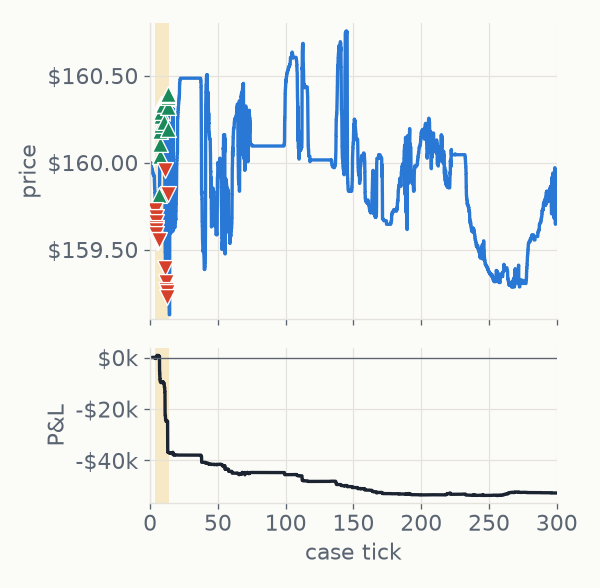
\includegraphics[width=\linewidth]{figures/J_CNR.png}\caption{CNR: $-\$53$k}\end{subfigure}\hfill
\begin{subfigure}{0.31\textwidth}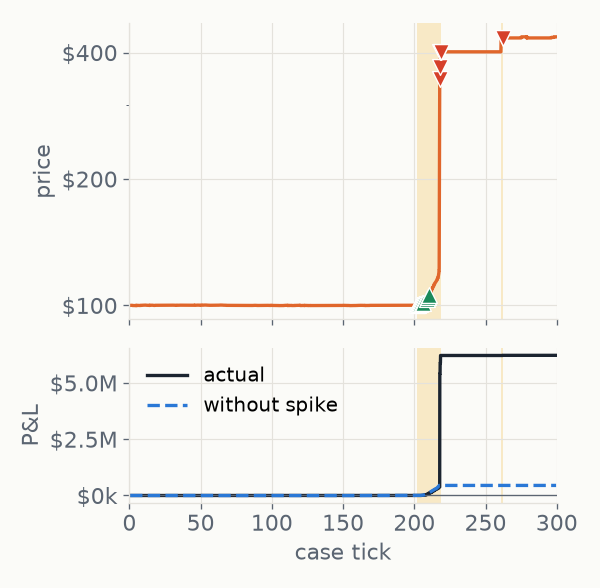
\includegraphics[width=\linewidth]{figures/J_RY.png}\caption{RY: $+\$6.22$M}\end{subfigure}\hfill
\begin{subfigure}{0.31\textwidth}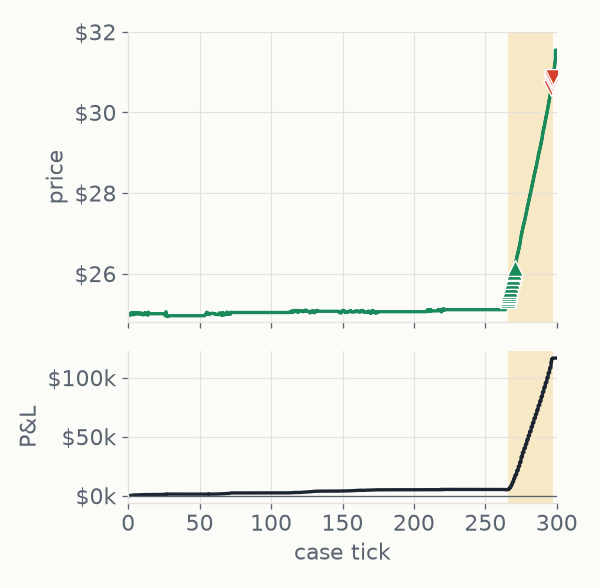
\includegraphics[width=\linewidth]{figures/J_AC.png}\caption{AC: $+\$117$k}\end{subfigure}
\caption{Price (top) and cumulative P\&L (bottom) per stock. Triangles: trend buys/sells; shading: trend mode; dashed (RY): P\&L without the tick-217 event.}
\label{fig:sec}
\end{figure}

\begin{itemize}
  \item \textbf{CNR, ticks 3--13:} three trend entries reversed at once ($-\$36.7$k). The opening book was thin (spreads of 11--100 ticks) and the volatility estimate had not warmed up,
        so noise looked like a trend. The adaptive threshold then worked: each loss raised CNR's entry bar $1.4\times$, three losses locked it out, and it never fired on CNR again.
        The \$40k circuit breaker fired once, at tick 38.
  \item \textbf{RY, ticks 200--217:} the efficiency ratio jumped from 0 to 1.0 at tick 200; at tick 201.6 the EMA gap held above 12 ticks and the engine bought 22{,}062 shares
        (88\% of the limit) at \$100.2--105.5, riding the drift to \$118. At tick 217 the book turned one-sided (asks vanished, bids at \$346 then \$402, following Group~12's activity);
        the engine sold everything in five orders over about four seconds, averaging roughly \$383.
  \item \textbf{AC, ticks 265--296:} entered at the start of a climb from \$25.1 to \$31.5, held about 22{,}000 shares, closed in the end-of-case unwind.
\end{itemize}

\textbf{Why market making did not pay, even with mean reversion.} The spread was one tick, so a winning round trip earns about \$0.01 per share plus rebate, while the inventory stop
is $\max(5\text{ ticks},3\sigma)$. At $+1$ tick per win and about $-5$ per stop, it needs roughly five wins in six to break even; prices moved in multi-cent jumps (86 stops on CNR) and
adverse selection meant fills clustered before moves. Mean reversion in the price is not the same as profitable market making.

\textbf{Size strategy: big only when evidence is strong or risk is small.}

\vspace{-2pt}
\begin{table}[H]
\centering\footnotesize
\begin{tabularx}{\textwidth}{lX}
\toprule
Market making & 5{,}000 shares/side when calm or in a 2--6 tick spread; 3{,}000 normally; half when stressed; 2{,}000 in thin books.\\
Inventory brake & $r=|\text{pos}|/9{,}000$: adding side $\times e^{-3r}$ and faded $\operatorname{round}(4r^{1.5})$ ticks; off at $r\ge0.85$; reducing side $\times(1+r)$ (Avellaneda--Stoikov-style skew).\\
Trend engine & First order 60\% of available cap, growing to 95\% (about 22{,}000 shares), orders of at most 5{,}000.\\
Limits \& unwind & Pre-trade worst-case cap 93\%; safety net cuts the largest position above 96\%; \$40k drawdown breaker; stop adding $\sim$20\,s before close, flat by $\sim$8\,s.\\
\bottomrule
\end{tabularx}
\end{table}
\vspace{-4pt}
Peak gross position over the run was 23{,}088 (net 22{,}837) against the 25{,}000 limit.

\textbf{Our Python script.} \code{algo2e\_fin.py} (submitted) needs Python 3 and \code{requests}. Start RIT with the API enabled, then:
\begin{lstlisting}
python algo2e_fin.py <API_KEY> <PORT> [CASE_MINUTES]     # e.g. python algo2e_fin.py abcde 15000 20
python algo2e_fin.py --mock whipsaw --seconds 90           # offline test, no RIT needed
\end{lstlisting}
If started early it waits until the case is \code{ACTIVE}; without \code{CASE\_MINUTES} it learns the clock. Options: \code{--no-dir} (market making only),
\code{--size N}, \code{--no-flatten-on-exit}; any constant can be overridden via \code{CFG\_<NAME>}. Ctrl-C cancels all orders and flattens. It prints fills, mode changes and a
per-second status line, and writes \code{logs/v3\_ticks\_*.csv} (one row per loop) and \code{logs/v3\_events\_*.csv} (every order and decision), which are the source of all numbers here.
\code{dir.py} (trend only) and \code{mm.py} (market making only) are the same code with one engine disabled.

The built-in mock exchange reproduces RIT's latency, position lag and fees across eleven scenarios. Re-running the final script on each (90\,s) gives: calm, mean-reverting and slow-grind
markets $-\$932$ to $+\$440$; trend, arch, reversal and crash $+\$41$k to $+\$124$k; spike, sweep and flood $+\$12$k to $+\$49$k; whipsaw $-\$44$k. Every run ended flat with peak gross
$\le$ 23{,}200. The shape matches the live result, and the whipsaw case is the same failure as CNR's opening.

\textbf{A note on the following round.} In the next round our RIT client crashed, so we had cancelled the script and only started it after the round was under way (first joining at
tick 49 of 300). It could not run the strategy as designed and the late session ended with a small loss of \$3{,}427. We mention it for completeness only.

%==========================================================================================
\q{(d) What was your P\&L?}

\textbf{\$6,288,771} for the main strategy (server net liquidation value, equal to the sum of the three stocks' P\&L to the cent, consistent with no fines). The variants ran on
separate accounts in the same market:

\vspace{-2pt}
\begin{table}[H]
\centering\footnotesize
\begin{tabular}{lrrrr}
\toprule
 & CNR & RY & AC & Total\\
\midrule
\code{algo2e\_fin.py} (market making + trend) & $-\$52{,}646$ & $\$6{,}224{,}827$ & $\$116{,}590$ & \textbf{\$6,288,771}\\
\code{dir.py} (trend only) & $-\$77{,}895$ & $\$6{,}238{,}173$ & $\$118{,}130$ & \$6,278,408\\
Market making only & $-\$28{,}719$ & $-\$6{,}147$ & $\$6{,}434$ & $-\$28{,}433$\\
\bottomrule
\end{tabular}
\end{table}
\vspace{-6pt}

\begin{figure}[H]
\centering
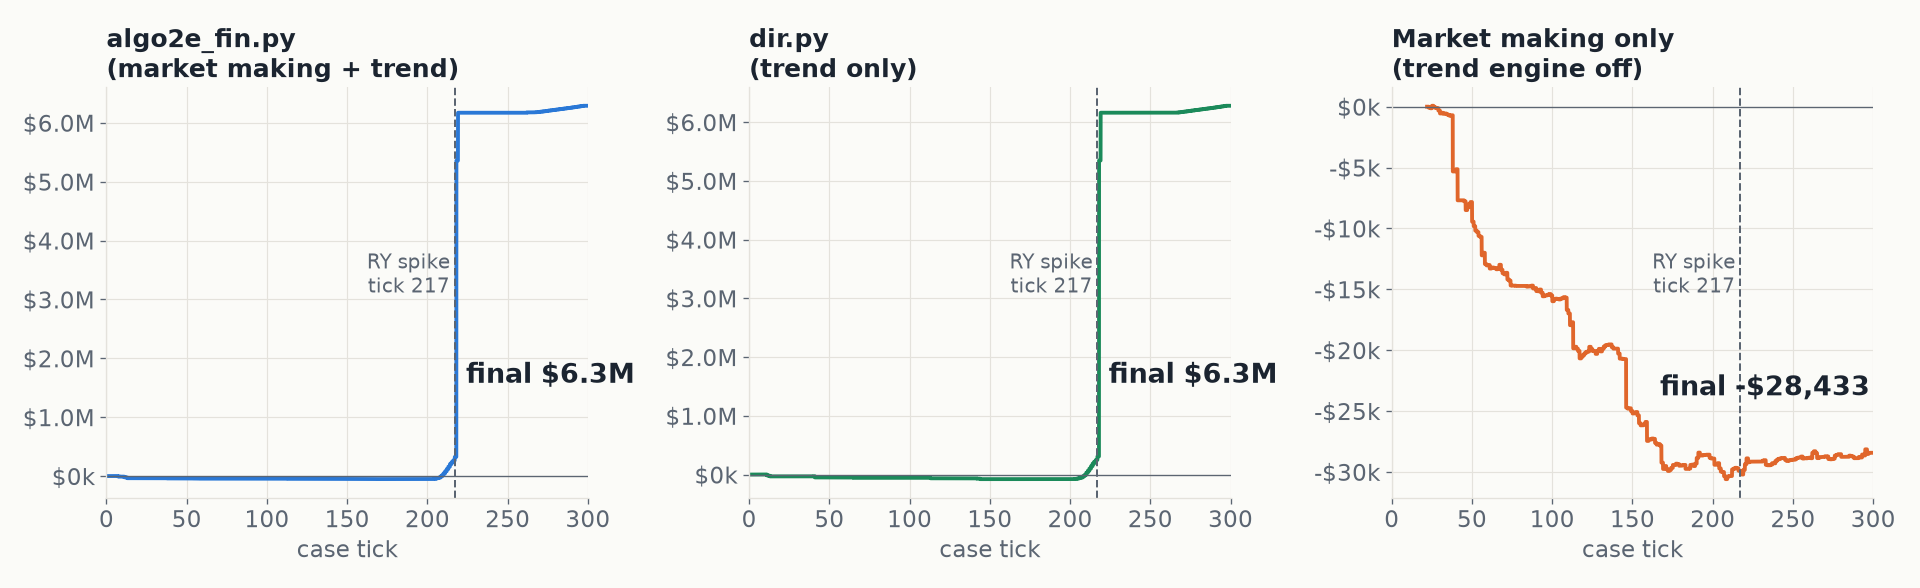
\includegraphics[width=0.92\textwidth]{figures/H3_total_pnl_three_algos.png}
\caption{Total P\&L through the case for the three builds; dashed line: RY event at tick 217.}
\end{figure}
\vspace{-4pt}

\textbf{Attribution.} The trend engine was in control less than 7\% of the time on any stock, yet earned $+\$6.30$M net: RY exit into the dislocation $+\$5.78$M, RY ride from \$100
$+\$451$k, AC $+\$112$k, CNR's early calls $-\$36$k. Market making, active the rest of the time, made about $-\$15$k. The builds confirm it: the same trend engine gives nearly the same
result with or without market making, while market making alone lost; \code{dir.py}'s earlier entries (8 vs.\ 12 ticks) cost it more on CNR.

\textbf{Without the RY event.} Re-valuing the RY exit at the last normal bid (\$121.08) gives about \textbf{\$511k} (\$244k--\$559k for exits between \$109 and \$123). This still includes
the drift before the event, so it is the optimistic reading; ticks 0--199 alone lost about \$52k.

\textbf{The mean-reversion tilt,} replayed on the logged signals, would have added about $+\$37$k (8{,}000 shares) or $+\$56$k (12{,}000) before costs, roughly $+\$5$--20k after, almost all
before tick 200 since it switches off in TREND. That is under 1\% of the total, consistent with leaving it off.

\textbf{Our reading.} We did not predict the RY event; the system put the right position on by rule before it happened and stayed within limits throughout. The run also showed what we would
fix first: a warm-up period before the trend engine may trade, and fee-aware quoting limited to stocks where resting earns a rebate.

\end{document}
